%\graphicspath{{~/Pictures/Screenshots/}}
\graphicspath{{~/Documents/MobAppDev/ThirdTask/img}}
\section*{\LARGE{Цель практической работы}}
\addcontentsline{toc}{section}{Цель практической работы}

\newpage

\section*{\LARGE{Выполнение практической работы}}
\addcontentsline{toc}{section}{Выполнение практической работы}

\section{Основы создания интерфейса}
При запуске приложения сначала запускается класс
MainActivity, который в качестве графического интерфейса устанавливает
разметку из файла activity\_main.xml. И поскольку в этой разметке прописан
элемент TextView, который представляет некоторый текст, то увидим
его текст на экране смартфона.

\subsection{Создание графического интерфейса}
Выполнение приложения Android по умолчанию начинается с класса
MainActivity, который по умолчанию открыт в Android Studio,
пример показан на рисунке \ref{fig:activity:start}.

\begin{figure}[h!tp]
	\centering
	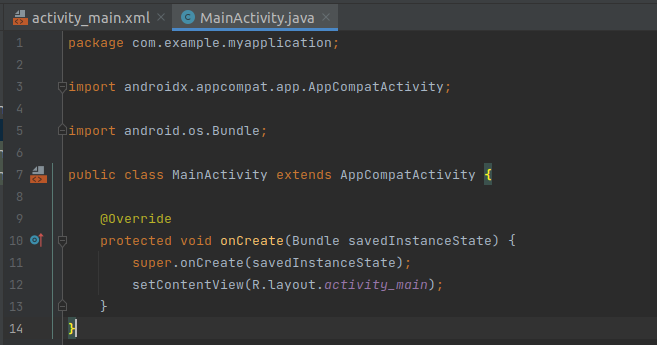
\includegraphics[width=0.6\textwidth]{Screenshot from 2023-03-09 17-16-57.png}
	\caption{Файл MainActivity.java}
	\label{fig:activity:start}
\end{figure}

Каждый отдельный экран или страница в приложении описывается таким
понятием как activity. В литературе могут использоваться различные
термины: экран, страница, активность.
Так вот, если запустить приложение на устройстве, то на экране появиться
определенную activity, которая предсталяет данный интерфейс.\par
Класс MainActivity, по сути, представляет обычный класс java, в начале
которого идет определение пакета данного класса.\par
Далее идет импорт классов из других пакетов, функциональность которых
используется в MainActivity.\par
По умолчанию MainActivity содержит только один метод \texttt{onCreate()}, в
котором фактически и создается весь интерфейс приложения.
В нем вызывается метод \texttt{setContentView()} передается ресурс разметки
графического интерфейса.
Именно здесь и решается, какой именно визуальный интерфейс будет иметь
MainActivity. Ресурс \texttt{R.layout.activity\_main} --- это файл
activity\_main.xml из каталога res/layout (в
принципе можно заметить, что название ресурса соответствует названию
файла), который также по умолчанию открыт в Android Studio.

\subsection{Файл activity\_main.xml}
Android Studio позволяет работать с визуальным интерфейсом как в режиме
кода, так и в графическом режиме. Так, по умолчанию файл открыт в
графическом режиме, и можно наглядно увидеть, как у примерно
будет выглядеть экран приложения.
Но также можно работать с файлом в режиме кода, поскольку
activity\_main.xml --- это обычный текстовый файл с разметкой xml. Для
переключения к коду нужно нажать на кнопку Code над графическим
представлением.\par
Разметка на уровне кода файл activity\_main.xml изображена
на рисунке \ref{fig:xml:layout}.

\begin{figure}[h!tp]
	\centering
	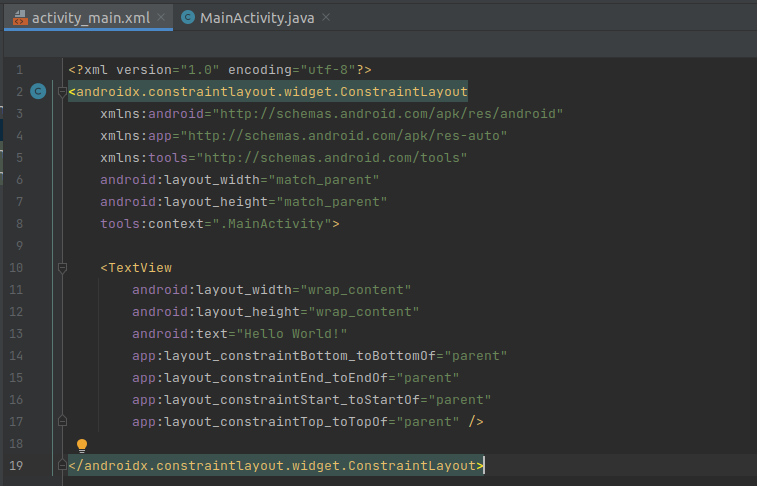
\includegraphics[width=0.8\textwidth]{Screenshot from 2023-03-09 17-29-58.png}
	\caption{Пример содержимого файла разметки}
	\label{fig:xml:layout}
\end{figure}

Весь интерфейс представлен элементом-контейнером
\texttt{androidx.constraintlayout.widget.ConstraintLayout}.\par
ConstraintLayout позволяет расположить вложенные элементы в
определенных местах экрана. Вначале элемента ConstraintLayout идет
определение пространств имен XML.
Каждое пространство имен задается следующим образом:
\texttt{xmlns:префикс="название\_ресурса"}.\par
Название ресурса (или URI - Uniform Resource Indicator) ---
\texttt{"http://schemas.android.com/apk/res/android"}.
И этот ресурс сопоставляется с префиксом android (\texttt{xmlns:android}).\par
Каждый ресурс или URI определяет некоторую функциональность,
которая используется в приложении, например, предоставляют теги и атрибуты,
которые необходимые для построения приложения:
\begin{itemize}
	\item \texttt{xmlns:android="http://schemas.android.com/apk/res/android"}:
		содержит основные атрибуты, которые предоставляются платформой
		Android, применяются в элементах управления и определяют
		их визуальные свойства (например, размер, позиционирование)
	\item \texttt{xmlns:app="http://schemas.android.com/apk/res-auto"}:
		содержит атрибуты, которые определены в рамках приложения
	\item \texttt{xmlns:tools="http://schemas.android.com/tools"}:
		применяется для работы с режиме дизайнера в Android Studio
\end{itemize}

И чтобы упростить работу с этими ресурсами, применяются префиксы.\par
\texttt{android:layout\_width} определяет ширину контейнера. Этот атрибут
(layout\_width) расположен в ресурсе
"http://schemas.android.com/apk/res/android". И поскольку этот ресурс
сопоставляется с префиксом android, то для обращения к атрибуту перед ним
через двоеточие указывается префикс данного ресурса.\par
Значением атрибута \texttt{android:layout\_weight} является
"match\_parent". Это значит, что элемент (ConstraintLayout)
будет растягиваться по всей ширине контейнера (экрана устройства).\par
Атрибут \texttt{android:layout\_height="match\_parent"} определяет высоту
контейнера и также определен в
"http://schemas.android.com/apk/res/android".\par
Значение "match\_parent" указывает, что ConstraintLayout
будет растягивается по всей длине контейнера (экрана устройства).\par
Атрибут \texttt{tools:context} определяет, какой класс
activity (экрана приложения) связан с текущим определением интерфейса.
В данном случае это класс MainActivity. Это позволяет использовать
в Android Studio различные возможности в режиме дизайнера,
которые зависят от класса activity.

\subsection{TextView}
Текстовое поле устанавливает текст с помощью атрибута android:text
(Рисунок \ref{fig:xml:textview}).

\begin{figure}[h!tp]
	\centering
	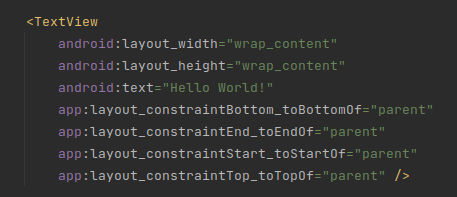
\includegraphics[width=0.8\textwidth]{Screenshot from 2023-03-09 17-49-55.png}
	\caption{Пример кода виджета TextView}
	\label{fig:xml:textview}
\end{figure}

\begin{description}
	\item[android:layout\_width] устанавливает ширину виджета. Значение
		wrap\_content задает для виджета величину, достаточную для
		отображения в контейнере.
	\item[android:layout\_height] устанавливает высоту виджета. Значение
		wrap\_content аналогично установке ширины задает для виджета высоту,
		достаточную для отображения в контейнере
	\item[android:text] устанавливает текст, который будет выводиться
		в TextView (в данном случае это строка "Hello World!")
	\item[app:layout\_constraintLeft\_toLeftOf="parent"] указывает, что левая
		граница элемента будет выравниваться по левой стороне контейнера
		ConstraintLayout
	\item[app:layout\_constraintTop\_toTopOf="parent"] указывает, что верхняя
		граница элемента будет выравниваться по верхней стороне контейнера
		ConstraintLayout
	\item[app:layout\_constraintRight\_toRightOf="parent"] указывает,
		что правая граница элемента будет выравниваться по правой стороне
		контейнера ConstraintLayout
\end{description}

\section{Создание интерфейса в коде java}
Для работы с визуальными элементами создадим новый проект. В качестве
шаблона проекта выберем Empty Activity.\par
Определим в классе MainActivity простейший интерфейс
(Рисунок~\ref{fig:activity:layout:java}).

\begin{figure}[h!tp]
	\centering
	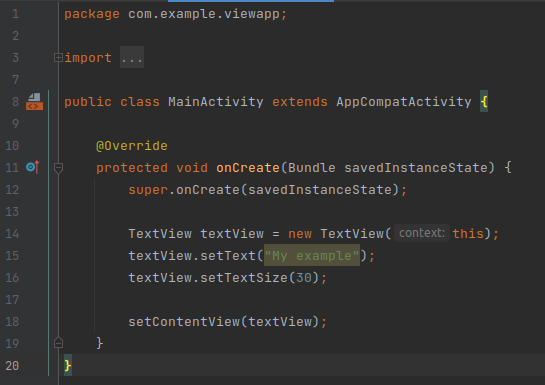
\includegraphics[width=0.8\textwidth]{Screenshot from 2023-03-09 18-10-05.png}
	\caption{Реализация интерфейса на джава}
	\label{fig:activity:layout:java}
\end{figure}

При создании виджетов в коде Java применяется их конструктор, в который
передается контекст данного виджета, а точнее объект
android.content.Context, в качестве которого выступает текущий класс
MainActivity.\par
Здесь весь интерфейс представлен элементом TextView, которое
предназначено для выводa текста. С помощью методов, которые, как
правило, начинаются на set, можно установить различные свойства TextView.
Например, в данном случае метод setText() устанавливает текст в поле, а
setTextSize() задает высоту шрифта.\par
Для установки элемента в качестве интерфейса приложения в коде Activity
вызывается метод setContentView(), в который передается визуальный
элемент.\par
Если запустить приложение, то получится визуальный интерфейс, показанный
на рисунку~\ref{fig:view:textview:java}.

\begin{figure}[h!tp]
	\centering
	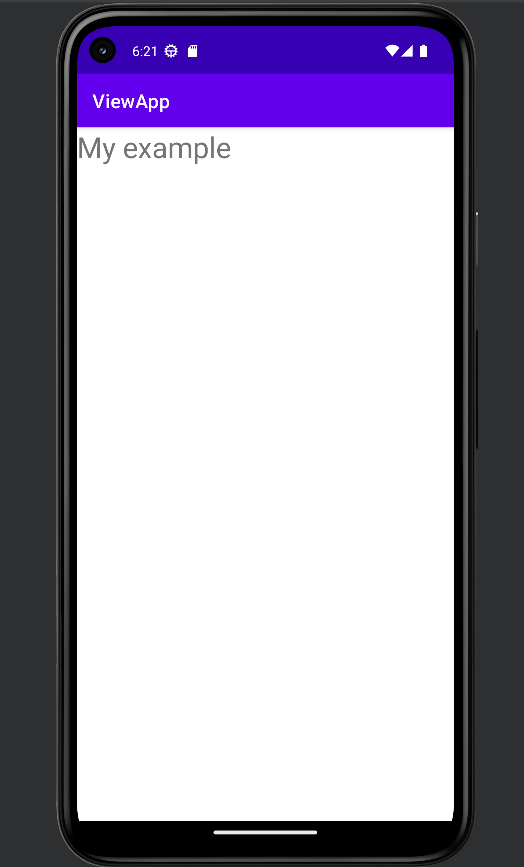
\includegraphics[width=0.8\textwidth]{Screenshot from 2023-03-09 18-21-21.png}
	\caption{Реализация интерфейса на джава}
	\label{fig:view:textview:java}
\end{figure}

\section{Определение интерфейса в файле XML}
Как правило, для определения визуального интерфейса в проектах под
Android используются специальные файлы xml. Эти файлы являются
ресурсами разметки и хранят определение визуального интерфейса в виде
кода XML. Подобный подход напоминает создание веб-сайтов, когда
интерфейс определяется в файлах html, а логика приложения - в коде
javascript.\par
Объявление пользовательского интерфейса в файлах XML позволяет
отделить интерфейс приложения от кода. Что означает, что мы можем
изменять определение интерфейса без изменения кода java. Например, в
приложении могут быть определены разметки в файлах XML для различных
ориентаций монитора, различных размеров устройств, различных языков и
т.д. Кроме того, объявление разметки в XML позволяет легче
визуализировать структуру интерфейса и облегчает отладку.\par
Файлы разметки графического интерфейса располагаются в проекте в
каталоге res/layout. По умолчанию при создании проекта с пустой activity уже
есть один файл ресурсов разметки activity\_main.xml, который может
выглядеть примерно так, как показано на рисунке~\ref{fig:xml:layout:d}.

\begin{figure}[h!tp]
	\centering
	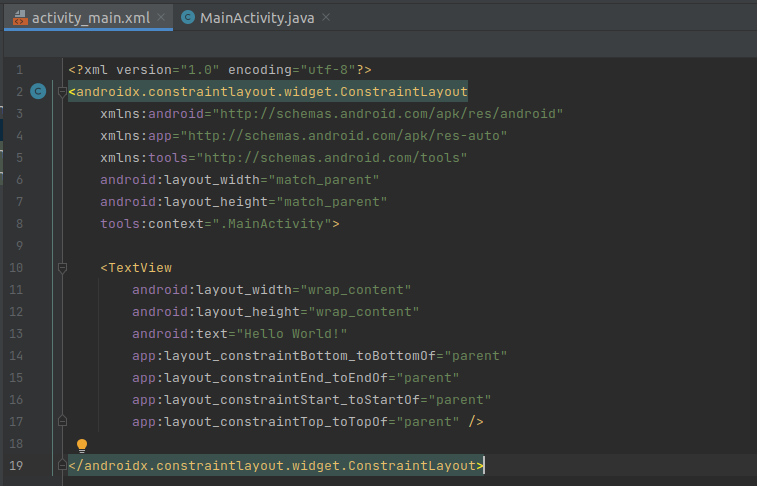
\includegraphics[width=0.8\textwidth]{Screenshot from 2023-03-09 17-29-58.png}
	\caption{Пример содержимого файла разметки}
	\label{fig:xml:layout:d}
\end{figure}

\section{Создание файла разметки}
В проекте может быть и несколько различных ресурсов layout. Как правило,
каждый отдельный класс Activity использует свой файл layout. Либо для
одного класса Activity может использоваться сразу несколько различных
файлов layout.\par
Добавили в проект новый файл разметки интерфейса. Для этого
нажали на каталок res/layout правой кнопкой мыши и в появившемся меню
выбрали пункт \texttt{New -> Layout Resource File}, как показано
на рисунке~\ref{fig:xml:layout:create}.

\begin{figure}[h!tp]
	\centering
	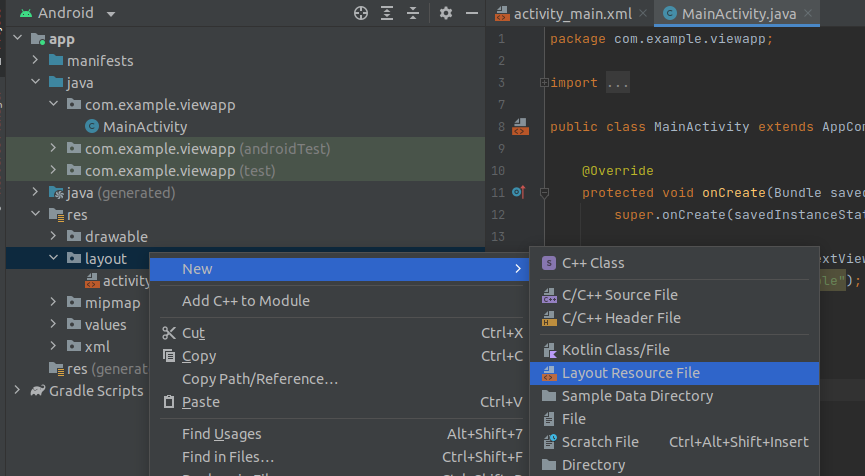
\includegraphics[width=0.8\textwidth]{Screenshot from 2023-03-10 11-25-24.png}
	\caption{Создание файла разметки}
	\label{fig:xml:layout::create}
\end{figure}

После этого в специальном окошке будет предложено указать имя и
корневой элемент для файла layout. И после нажатия на кнопку \texttt{Ok},
в каталог res/layout будет добавлен новый файл second\_layout.xml,
с которым мы можем работать точно также, как и с activity\_main.xml.\par

\section{Получение и управление визуальными элементами в коде}
Открыли файл second\_layout.xml и изменили его содержимое, как показано
на рисунке~\ref{fig:xml:textview:d}.

\begin{figure}[h!tp]
	\centering
	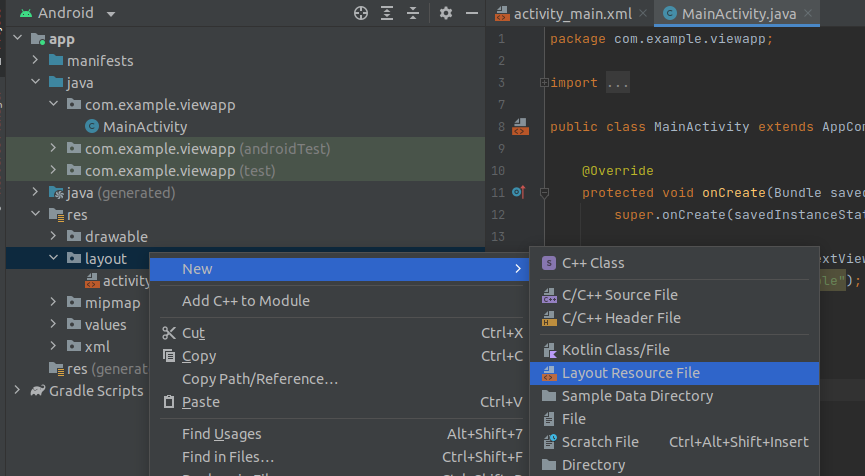
\includegraphics[width=0.8\textwidth]{Screenshot from 2023-03-10 11-25-24.png}
	\caption{Изменение файла second\_layout.xml}
	\label{fig:xml:textview:d}
\end{figure}

Здесь определено текстовое поле TextView, которое имеет
атрибут \texttt{android:id}~--- идентификатор элемента,
через можно будет ссылаться на него в коде.
В записи \texttt{android:id="@+id/header"} символ
\texttt{@} указывает XML-парсеру использовать оставшуюся часть строки
атрибута как идентификатор. А знак \texttt{+} означает, что если для
элемента не определен id со значением header, то его следует
определить.
Пример обращения из кода Джава к виджету через этот индентификатор в
классе MainActivity, показан на рисунке~\ref{fig:java:textview:manage}.

\begin{figure}[h!tp]
	\centering
	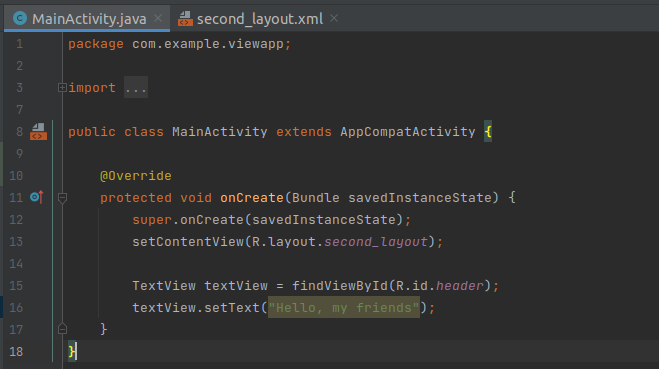
\includegraphics[width=0.8\textwidth]{Screenshot from 2023-03-10 11-49-06.png}
	\caption{Управление виджетом в коде Джава}
	\label{fig:java:textview:manage}
\end{figure}

С помощью метода setContentView() устанавливается разметка из файла
second\_layout.xml.\par
Другой важный момент, который стоит отметить --- получение визуального
элемента TextView. Так как в его коде определили атрибут \texttt{android:id},
то через этот id мы можем его получить.\par
Для получения элементов по id класс Activity имеет метод
\texttt{findViewById()}. В этот метод передается идентификатор ресурса в виде
\texttt{R.id.[идентификатор\_элемента]}. Этот метод возвращает объект View~---
объект базового класса для всех элементов, поэтому результат метода еще
необходимо привести к типу TextView.

\section{Определение размеров}
При разработке приложений под Android используются различные
типы измерений:
\begin{itemize}
	\item px: пиксели текущего экрана. Однако эта единица измерения не
		рекомендуется, так как реальное представление внешнего вида
		может изменяться в зависимости от устройства; каждое устройство
		имеет определенный набор пикселей на дюйм, поэтому количество
		пикселей на экране может также меняться
	\item dp: (device-independent pixels) независимые от плотности экрана
		пиксели. Абстрактная единица измерения, основанная на физической
		плотности экрана с разрешением 160 dpi (точек на дюйм).
		В этом случае 1dp = 1px. Если размер экрана больше или меньше,
		чем 160dpi, количество пикселей, которые применяются
		для отрисовки 1dp соответственно увеличивается или уменьшается.
		Например, на экране с 240 dpi 1dp=1,5px, а на экране с 320dpi 1dp=2px.
		Общая формула для получения количества физических пикселей
		из dp: \( px = dp * (dpi / 160) \).
	\item sp: (scale-independent pixels) независимые от масштабирования
		пиксели. Допускают настройку размеров, производимую
		пользователем. Рекомендуются для работы со шрифтами.
	\item pt: 1/72 дюйма, базируются на физических размерах экрана
	\item mm: миллиметры
	\item in: дюймы
\end{itemize}
Предпочтительными единицами для использования являются dp. Это связано
с тем, что мир мобильных устройств на Android сильно фрагментирован в
плане разрешения и размеров экрана. И чем больше плотность пикселей на
дюйм, тем соответственно больше пикселей будет доступно.\par
Используя же стандартные физические пиксели, можно столкнуться с
проблемой, что размеры элементов также будут сильно варьироваться в
зависимости от плотности пикселей устройства.\par
Для упрощения работы с размерами все размеры разбиты на несколько
групп:
\begin{itemize}
	\item ldpi (low): $\sim$120dpi;
	\item mdpi (medium): $\sim$160dpi;
	\item hdpi (high):
		$\sim$240dpi (к данной группе можно отнести такое древнее
		устройство как Nexus One);
	\item xhdpi (extra-high): $\sim$320dpi (Nexus 4);
	\item xxhdpi (extra-extra-high):
		$\sim$480dpi (Nexus 5/5X, Samsung Galaxy S5);
	\item xxxhdpi (extra-extra-extra-high):
		$\sim$640dpi (Nexus 6/6P, Samsung Galaxy S6).
\end{itemize}

\section{Установка размеров}
Основная проблема, связанная с размерами, связана с их установкой в коде
Java. Например, некоторые методы принимают в качестве значения
физические пиксели, а не device-independent pixels. В этом случае может
потребоваться перевести значения из одного типа единиц в другой. Для этого
требуется применить метод TypedValue.applyDimension().\par
Параметр unit представляет тип единиц, из которой надо получить значение в
пикселях. Тип единиц описывается одной из констант TypedValue:
\begin{itemize}
	\item COMPLEX\_UNIT\_DIP - dp или независимые от плотности экрана пиксели;
	\item COMPLEX\_UNIT\_IN - in или дюймы;
	\item COMPLEX\_UNIT\_MM - mm или миллиметры;
	\item COMPLEX\_UNIT\_PT - pt или точки;
	\item COMPLEX\_UNIT\_PX - px или физические пиксели;
	\item COMPLEX\_UNIT\_SP - sp или независимые от масштабирования
		пиксели (scale-independent pixels).
\end{itemize}
Параметр value представляет значение, которое надо преобразовать.
Параметр metrics представляет информацию о метрике, в рамках которой
надо выполнить преобразование.\par
В итоге метод возвращает преобразованное значение. 
Для примера получили из 30dp обычные физические пиксели
(Рисунок~\ref{fig:java:applydim}).

\begin{figure}[h!tp]
	\centering
	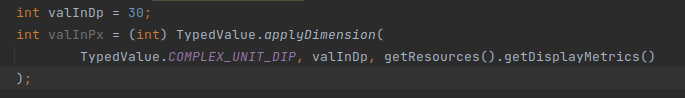
\includegraphics[width=0.8\textwidth]{Screenshot from 2023-03-10 12-28-01.png}
	\caption{Пример перевода единиц измерения разметки}
	\label{fig:java:applydim}
\end{figure}

В качестве третьего аргумента передается вызов метода
getResources().getDisplayMetrics(), который позволяет получить информацию
о метрике, связанной с текущим устройством. В итоге получили из 30dp
некоторое количество пикселей.

\section{Ширина и высота элементов}
Все визуальные элеметы, которые мы используем в приложении, как
правило, упорядочиваются на экране с помощью контейнеров. В Android
подобными контейнерами служат такие классы как RelativeLayout,
LinearLayout, GridLayout, TableLayout, ConstraintLayout, FrameLayout. Все
они по разному располагают элементы и управляют ими, но есть некоторые
общие моменты при компоновке визуальных компонентов, которые мы
сейчас рассмотрим.
Для организации элементов внутри контейнера используются параметры
разметки. Для их задания в файле xml используются атрибуты, которые
начинаются с префикса layout\_. В частности, к таким параметрам относятся
атрибуты layout\_height и layout\_width, которые используются для установки
размеров и могут использовать одну из следующих опций:
\begin{itemize}
	\item Растяжение по всей ширине или высоте контейнера с помощью значения
		match\_parent (для всех контейнеров кроме ConstraintLayout)
		или 0dp (для ConstraintLayout);
	\item Растяжение элемента до тех границ, которые достаточны,
		чтобы вместить все его содержимое с помощью значения wrap\_content.
\end{itemize}

\subsection{match\_parent}
Установка значения match\_parent позволяет растянуть элемент по всей
ширине или высоте контейнера. Стоит отметить, что данное значение
применяется ко всем контейнерам, кроме ConstraintLayout. Например,
элемент TextView имеет значения
\texttt{android:layout\_width="match\_parent"}, обеспечивающее растяжение
по ширине, а \texttt{android:layout\_height="match\_parent"}~--- по вертикали.
Для наглядности в TextView применяет атрибут android:background,
который представляет фон и в данном случае окрашивает элемент
в цвет "<\#FFBB86FC">, благодаря чему можно увидеть занимаемую им область
(Рисунок~\ref{fig:xm:set_hw}).

\begin{figure}[h!tp]
	\centering
	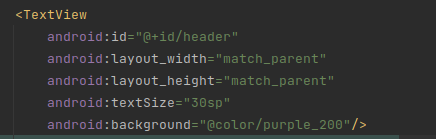
\includegraphics[width=0.8\textwidth]{Screenshot from 2023-03-10 12-42-04.png}
	\caption{Использование агрумента match\_parent}
	\label{fig:xm:set_hw}
\end{figure}

\subsection{wrap\_content}
Значение wrap\_content устанавливает те значения для ширины или высоты,
которые необходимы, чтобы разместить на экране содержимое элемента.

\section{Программная установка ширины и высоты}
Если элемент, к примеру, тот же TextView создается в коде java, то для
установки высоты и ширины можно использовать метод setLayoutParams().
Так, как показано на рисунке~\ref{fig:java:set_hw}.

\begin{figure}[h!tp]
	\centering
	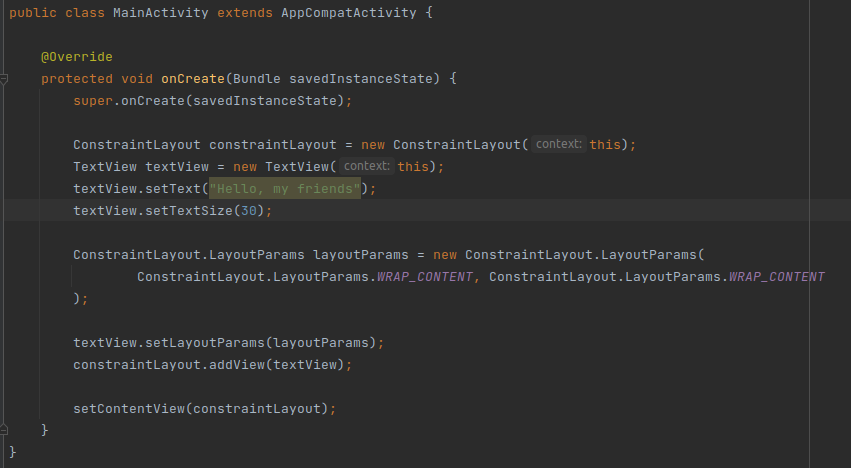
\includegraphics[width=0.9\textwidth]{Screenshot from 2023-03-10 12-53-59.png}
	\caption{Установка ширины и высоты в коде Джава}
	\label{fig:java:set_hw}
\end{figure}

В метод \texttt{setLayoutParams()} передается объект ViewGroup.LayoutParams.
Этот объект инициализируется двумя параметрами: шириной и высотой.
Для указания ширины и высоты можно использовать одну из констант
\texttt{ViewGroup.LayoutParams.WRAP\_CONTENT} или
\texttt{ViewGroup.LayoutParams.MATCH\_PARENT} (в случае с LinearLayout или
RelativeLayout).

\section{Внутренние и внешние отступы}
Параметры разметки позволяют задать отступы как от внешних границ
элемента до границ контейнера, так и внутри самого элемента между его
границами и содержимым.

\subsection{Padding}
Для установки внутренних отступов применяется атрибут
\texttt{android:padding}. Он устанавливает отступы контента от всех четырех
сторон контейнера. Можно устанавливать отступы только от одной стороны
контейнера, применяя следующие атрибуты:
\texttt{android:paddingLeft, android:paddingRight,
android:paddingTop} и \texttt{android:paddingBottom}.
Пример использования этого атрибута показан на рисунке~\ref{fig:xml:padding}.

\begin{figure}[h!tp]
	\centering
	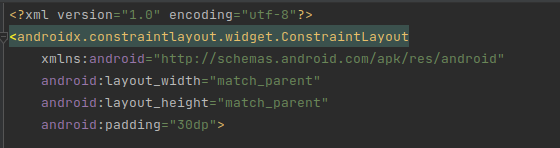
\includegraphics[width=0.9\textwidth]{Screenshot from 2023-03-10 13-01-54.png}
	\caption{Использование padding в разметке}
	\label{fig:xml:padding}
\end{figure}

\subsection{Margin}
Для установки внешних отступов используется атрибут \texttt{layout\_margin}.
Данный атрибут имеет модификации, которые позволяют задать отступ
только от одной стороны: \texttt{android:layout\_marginBottom,
android:layout\_marginTop, android:layout\_marginLeft} и
\texttt{android:layout\_marginRight} (отступы соответственно от нижней,
верхней, левой и правой границ).
Пример использования этого атрибута показан на рисунке~\ref{fig:xml:margin}.

\begin{figure}[h!tp]
	\centering
	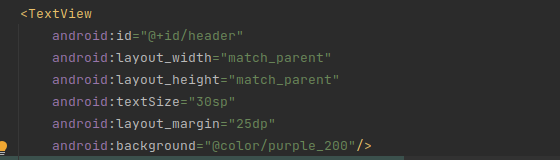
\includegraphics[width=0.9\textwidth]{Screenshot from 2023-03-10 13-08-23.png}
	\caption{Использование padding в разметке}
	\label{fig:xml:margin}
\end{figure}

\section{Программная установка отступов}
Для программной установки внутренних отступов у элементы вызывается
метод \texttt{setPadding(left, top, right, bottom)},
в который передаются четыре значения для каждой из сторон.
Также можно по отдельности задать отступы с помощью методов
\texttt{getPaddingLeft(), getPaddingTop(), getPaddingRight()} и
\texttt{getPaddingBottom()}.
Для установки внешних отступов необходимо реализовать объект
LayoutParams для того контейнера, который применяется.
И затем вызвать у этого объекта LayoutParams метод
\texttt{setMargins(left, top, right, bottom)}.
Пример использования этих методов показан на рисунке~\ref{fig:java:pd_mrg}.

\begin{figure}[h!tp]
	\centering
	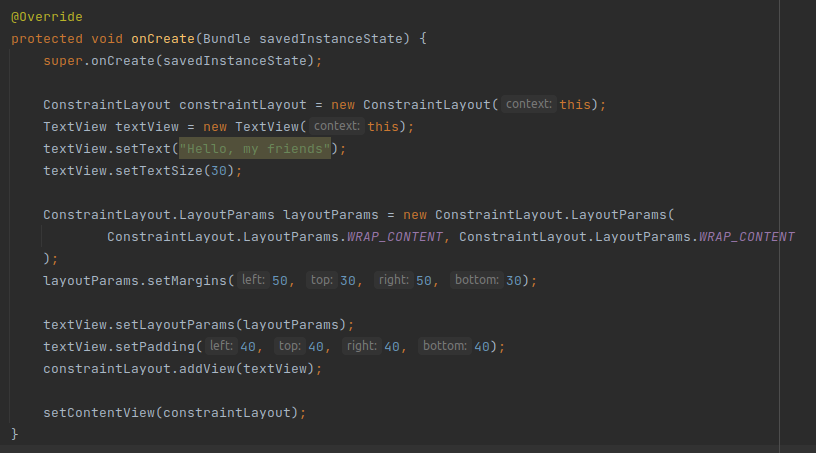
\includegraphics[width=0.9\textwidth]{Screenshot from 2023-03-10 13-16-40.png}
	\caption{Использование padding в разметке}
	\label{fig:java:pd_mrg}
\end{figure}


%13.Реализуйте примеры применения контейнера ConstraintLayout.
%(позиционирование,сдвиг, горизонтальная цепочка элементов, вес
%элемента, горизонтальный ряд виджетов, вертикальная цепочка,
%программное создание ConstraintLayout )

